%\subsection{Event Slicing and Cosmic Removal in Pandora}
The work presented in this note relies on the Pandora event reconstruction~\cite{bib:pandoraub}. Pandora does the low-level pattern-recognition step of the reconstruction, i.e. groups hits into clusters, clusters into particles and particles into hierarchies. This section focuses on the cosmic rejection aspect of the analysis. We describe here how the output of Pandora's pattern-recognition is combined with scintillation light to isolate possible candidate neutrino interactions in MicroBooNE. This process is illustrated in the three images of Figure~\ref{fig:sliceid}. Moreover, we describe how the additional information from the Cosmic Ray Tagger (CRT) is used to improve cosmic rejection in the \numu selection. 

\begin{figure}[ht] 
\begin{center}
    \begin{subfigure}[b]{0.7\textwidth}
    \centering
    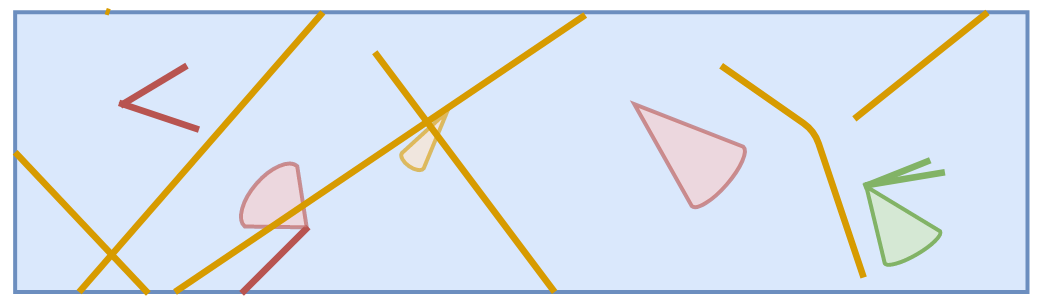
\includegraphics[width=1.00\textwidth]{NuId-Ch3/Images/slice00.png}
    \caption{\label{fig:slcieid:00} Typical event with multiple interactions isolated by Pandora in \texttt{slices}. Candidate neutrino interactions are shown in green and red.  Obvious cosmics are shown in orange.}
    \end{subfigure}
    \begin{subfigure}[b]{0.7\textwidth}
    \centering
    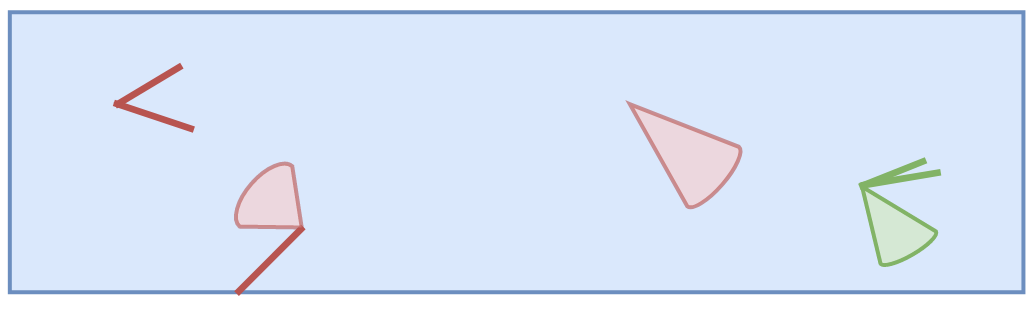
\includegraphics[width=1.00\textwidth]{NuId-Ch3/Images/slice01.png}
    \caption{\label{fig:slcieid:01} Event after the removal of \texttt{obvious cosmics} tagged geometrically by Pandora.}
    \end{subfigure}
    \begin{subfigure}[b]{0.7\textwidth}
    \centering
    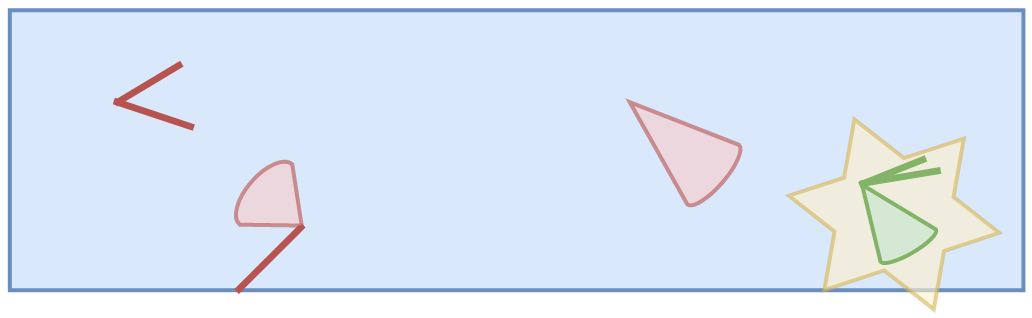
\includegraphics[width=1.00\textwidth]{NuId-Ch3/Images/slice02.png}
    \caption{\label{fig:slcieid:02} Implementation of the \texttt{SiceID} tool to isolate possible candidate $\nu$ interactions.  The selected candidate is highlighted, and shown in green.}
    \end{subfigure}
\caption{\label{fig:sliceid} Succession of steps in cosmic removal performed using Pandora's topological pattern recognition combined with scintillation light information through the \texttt{NeutrinoID} tool.}
\end{center}
\end{figure}

%\subsection{Slicing, Clustering and Vertexing}
\subsection{Pandora Slicing, Clustering and Vertexing}
The creation of a ``slice" is the first step of the Pandora processing. A slice is a collection of distinct reconstructed particles which belong to the same interaction, such as a cosmic muon and its Michel electron, or the muon and proton in a 1$\mu$1$p$ neutrino interaction. To produce slices, the Pandora cosmic pattern recognition is first run over all hits, aiming to construct muon tracks and any associated $\delta$-rays or Michel electrons under the cosmic hypothesis (fig.~\ref{fig:slcieid:00}). At this stage, obvious cosmic activity (through-going or out-of-time muons) is tagged using geometric information and discarded (fig.~\ref{fig:slcieid:01}). The remaining hit collection is used as input to Pandora and reconstructed both under the cosmic hypothesis and the neutrino hypothesis. A typical event contains approximately five slices at this stage. 

%\subsubsection{Clustering and Vertex Finding } 
\par In order to reconstruct the interactions in three dimensions, Pandora needs to match the information from at least two different views and create a neutrino vertex. Pandora performs the 2D clustering on the hits in each slice and on each plane separately. Then a number of 3D candidate vertices is created by finding positions that project down onto the ends of the available 2D clusters. All of the possible vertex candidates are fed into the support vector machine (SVM) vertex selection, and the candidate with the highest SVM score is chosen. This 3D vertex is used to split any existing clusters that cover the vertex. Then the cluster matching algorithms are run; in these algorithms the clusters are compared between views and modified to improve the matching.

\subsection{Pandora NeutrinoID: Cosmic Removal Via Topology and Scintillation Light}
\label{sec:sliceID:NeutrinoID}
\par After the set of Pandora pattern-recognition algorithms has isolated individual interactions into reconstructed slices and removed obvious cosmics, the remaining task is to identify which slice, if any, is associated with a neutrino interaction. Scintillation light information is used to reject slices incompatible with light recorded in-time with the beam. Topological cuts aimed at rejecting stopping-muon events which enter the TPC are also used. The \texttt{NeutrinoID} is at the core of all neutrino selections performed in this analysis; this first, common step is responsible for the majority of cosmic-rejection.
\\
\par We leverage three handles to distinguish between neutrino and cosmic-ray slices:
\begin{enumerate}
    \item Simple optical pre-selection cuts, which remove slices inconsistent with the beam flash;
    \item A topological score which assesses to what extent the slice looks like a neutrino interaction in the TPC (see DocDB 14175)
    \item A flash-matching score, which assesses how well the flash-hypothesis for the slice matches the beam flash.
\end{enumerate}

To select the neutrino slice, we first require a beam-triggered flash in the beam window. Then we apply the optical pre-selection cuts. If no slice passes optical pre-selection, the event is rejected. If the slice with the largest topological score passes the optical pre-selection, the slice forms the neutrino candidate; otherwise, the slice with the largest  flash-matching score forms the neutrino candidate. 
The performance of the \texttt{NeutrinoID} for simulated neutrino events is shown in~\cref{fig:sliceid_eff}.
Integrated over all final states and neutrino energies, the efficiency is:
\begin{itemize}
    \item[-] $\nu_\mu$ charged-current: \SI{83.0}{\%}
    \item[-] $\nu_e$ charged-current: \SI{83.3}{\%}
\end{itemize}
Further details on the \texttt{NeutrinoID} tool are available in DocDB 28418, 23854 and 22519.

\begin{figure}[H]
    \centering
    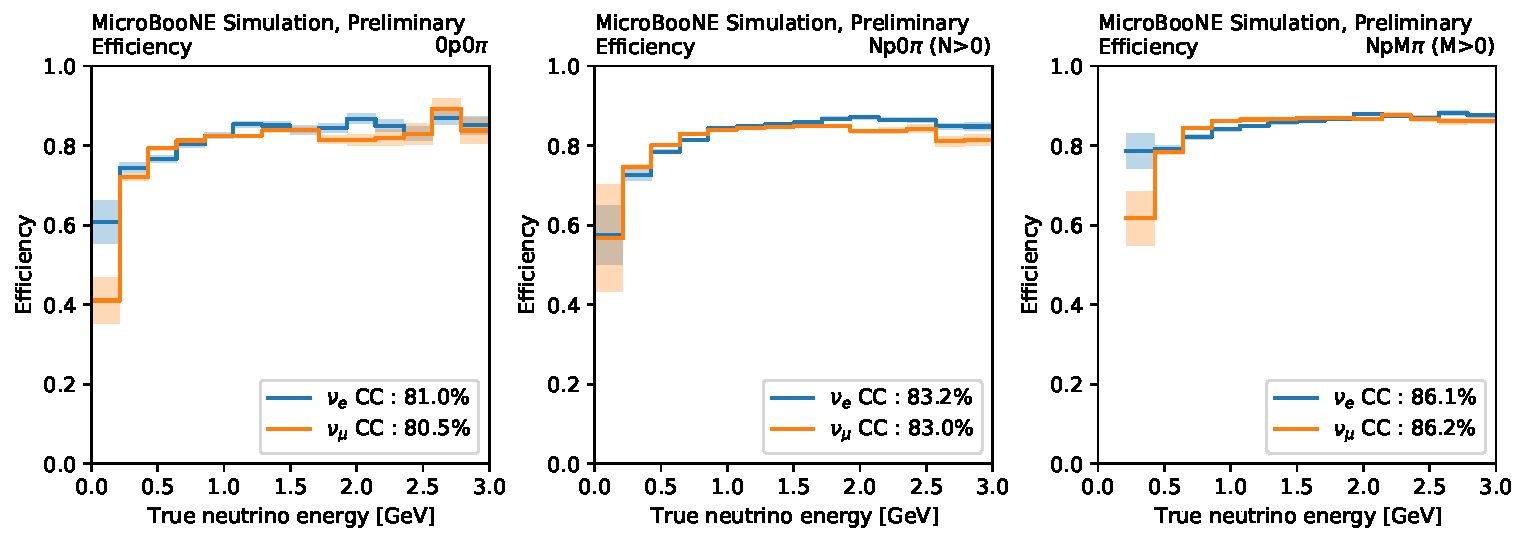
\includegraphics[width=0.75\textwidth]{NueCCsel/Images/truth/sliceID_eff.pdf}
    \caption{The performance of the \texttt{NeutrinoID} tool as a function of the true neutrino energy for the topologies considered in the \nuecc selection: \zpsel (left), \npsel (middle) and inclusive (right) channels. The energy range is \SIrange{0}{3}{\GeV} and the bin size is \SI{200}{\MeV}. The shaded areas correspond to the statistical errors arising from limiter simulated sample sizes.}
    \label{fig:sliceid_eff}
\end{figure}



\subsection{CRT Veto and Distance Tagger}
\label{sec:sliceID:CRT}
CRT tools are used in this analysis to boost cosmic rejection in the $\nu_{\mu}$ constrain selection, where the analysis-level containment requirement removes the concern of tagging exiting muons through CRT-based cuts. CRT-based cuts were explored for the $\nu_e$ selections as well but were ultimately found to be of little impact in the \npsel due to the powerful cosmic rejection achieved when requiring final-state protons. Considerable additional cosmic rejection was obatined with the CRT in the \zpsel, but the current analysis has chosen to not implement these cuts to avoid complications in mixing datasets from different runs with different selection requirements. Two specific cut concepts have been developed to make use of CRT information. Both are used in the $\nu_{\mu}$ and are described below.

\textbf{CRT Veto.} The CRT veto looks for a time coincidence between the scintillation light recorded in time with the 1.6 $\mu$s beam-spill (beam flash) and a CRT hit: if a CRT hit occurs within 1 $\mu s$ of the beam flash, the event is rejected. For this coincidence, only CRT hits with PE $>$ 100 p.e. are considered; we do not apply a constraint on the position of the flash or on the position of the CRT hit. 
The rejection power and efficiency of the CRT veto are calculated using the BNB external and the $\nu_e$ overlay samples, respectively. The BNB external rejection rate is $\sim$59\%. %,  and the $\nu_e$ passing rate greater than $\sim$94\% for all electron neutrino energies, even higher at low energies. \\

\textbf{CRT Distance Tagger.} 
The CRT Distance Tagger tool builds upon the standard Pandora neutrino vertex reconstruction and the CRT tagging of TPC tracks. A TPC track is tagged with a CRT hit association if the track projection onto a CRT panel and a CRT hit are close in space. 
To perform this association, the track projection to the CRT is calculated under the hypothesis that the associated particle crossed the TPC at the time registered by the CRT hit under consideration. More details on the CRT hit to TPC track matching are available in \cite{bib:CRTPresel_Technote}.  The CRT Distance Tagger checks the minimum distance between the reconstructed neutrino vertex and each track tagged with a CRT hit. If the minimum distance is less than 14 cm, the event is rejected. An example event tagged by this cut is shown in Figure~\ref{fig:crtdist00}.  With the CRT Distance Tagger an additional 19\% of off-beam backgrounds are rejected.% external passing rate is $\sim$81\%,  and the $\nu_e$ efficiency is greater than $\sim$96\% for all electron neutrino energies, even higher at low energies. \\
 
\begin{figure}[h!]
\centering
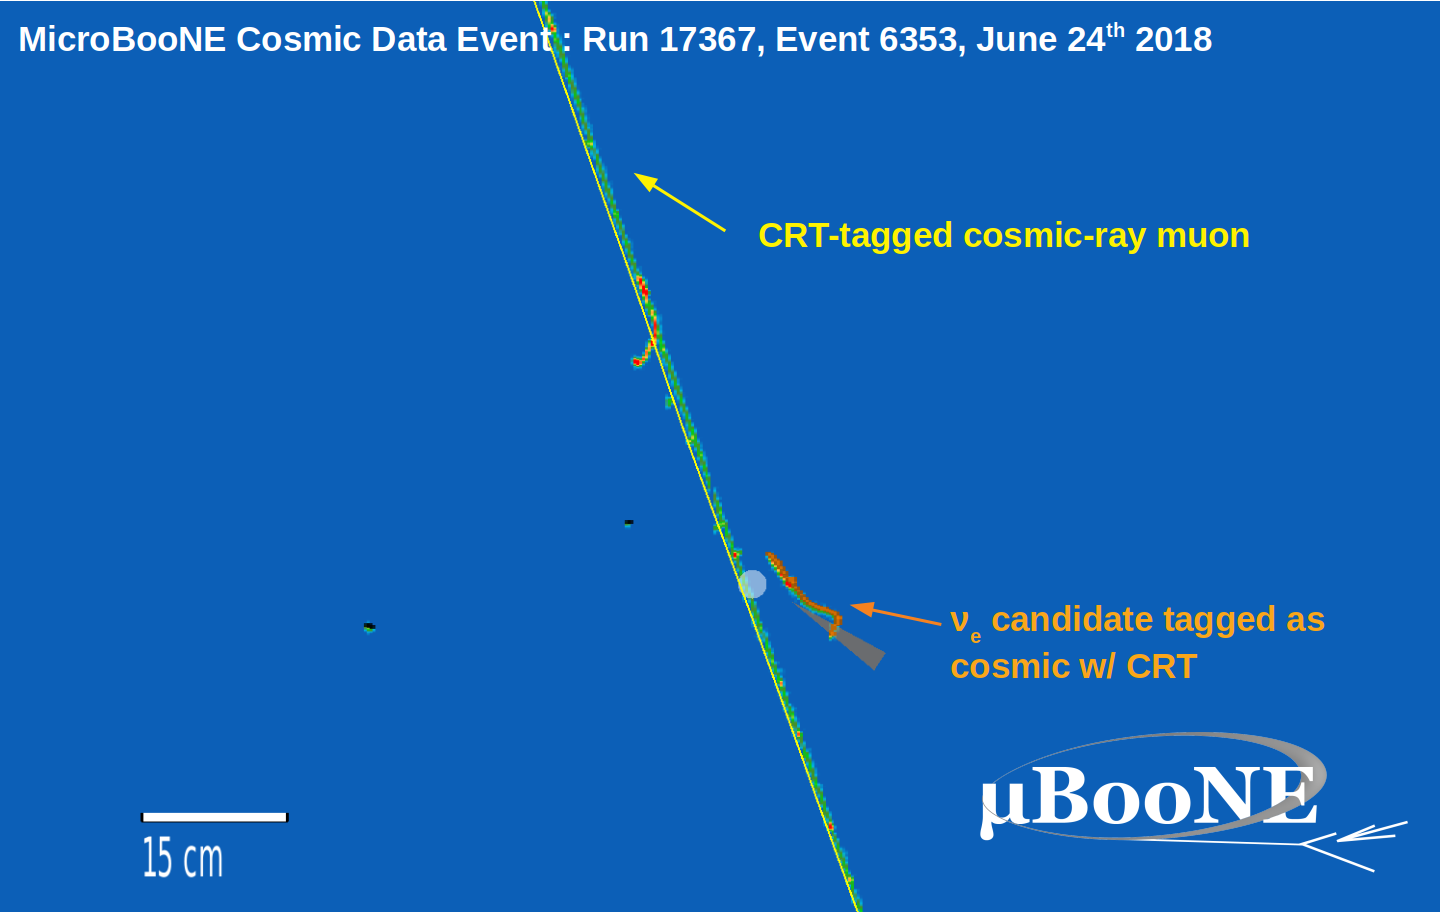
\includegraphics[width=0.4\textwidth]{NuId-Ch3/Images/crttagger_01.png}
\caption{Example $\nu_e$ candidate tagged as cosmic by the the CRT distance tagger. From the event one can see that the reconstructed EM shower is from EM activity that is associated with the cosmic muon.}
\label{fig:crtdist00}
\end{figure}

An overview of the impact of the CRT on cosmic rejection can be seen in Figure~\ref{fig:crt} where the beam-time distribution for the 8E18 POT Run 3 open data set is shown just after \texttt{NeutrinoID} (left), and after both \texttt{NeutrinoID} and CRT cosmic-tagging tools (including the CRT veto and distance tagger) have been applied (right). The EXT backgrounds drop by more than a factor of three, with an efficiency for $\nu_{\mu}$ CC contained interaction (at pre-selection stage, as defined in sec.~\ref{sec:NuMUCCsel}) of 90\%.
Further details and a preliminary study of the CRT  impact on an electron neutrino pre-selection can be found in \cite{bib:CRTPresel_Technote}. 

\begin{figure}[ht] 
\begin{center}
    \begin{subfigure}[b]{0.4\textwidth}
    \centering
    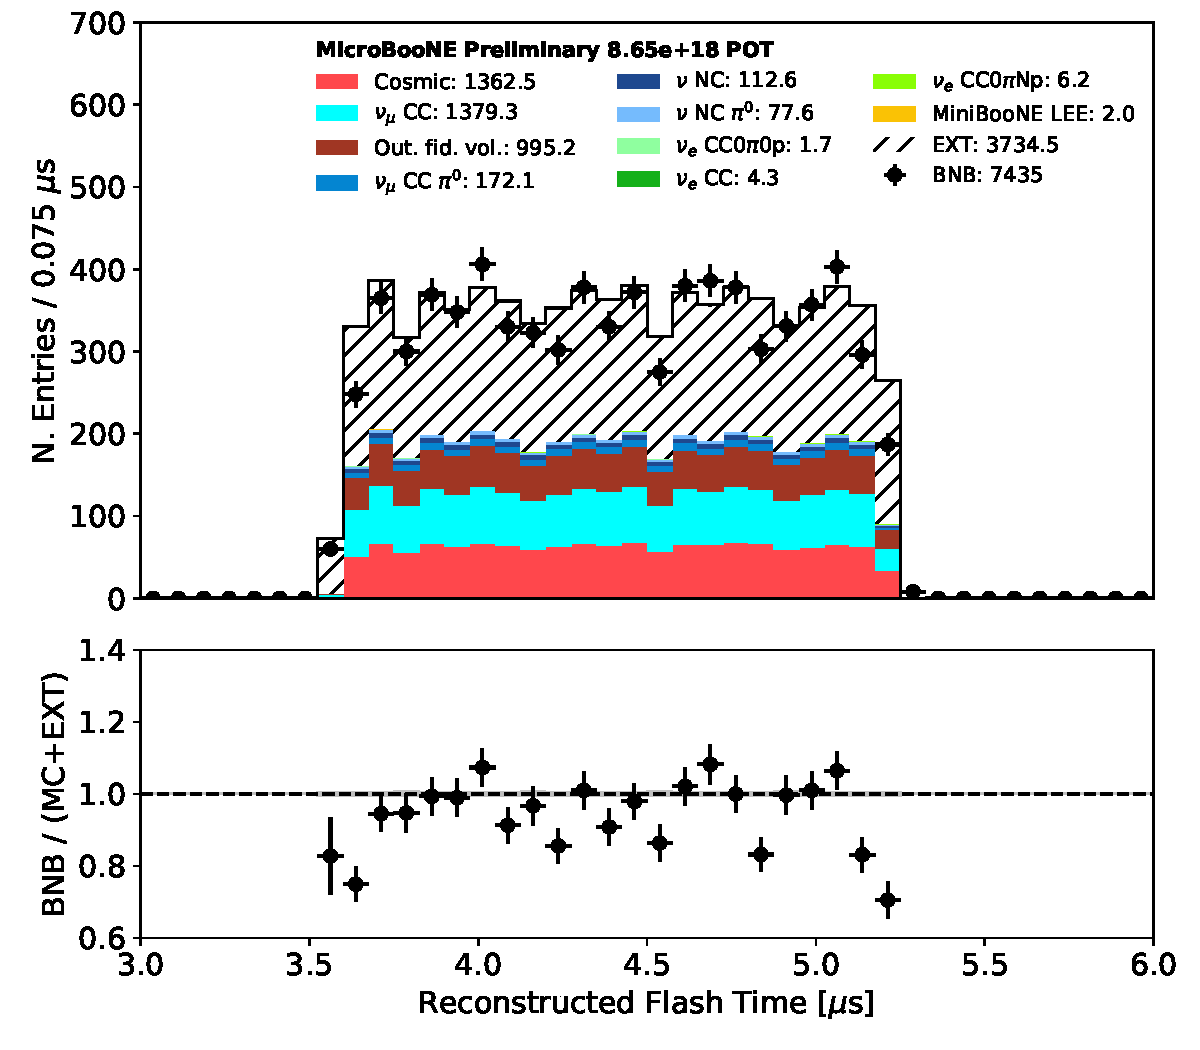
\includegraphics[width=1.00\textwidth]{NuId-Ch3/Images/flash_time_01152020.pdf}
    \caption{\label{fig:crt:pre} No CRT tools.}
    \end{subfigure}
    \begin{subfigure}[b]{0.4\textwidth}
    \centering
    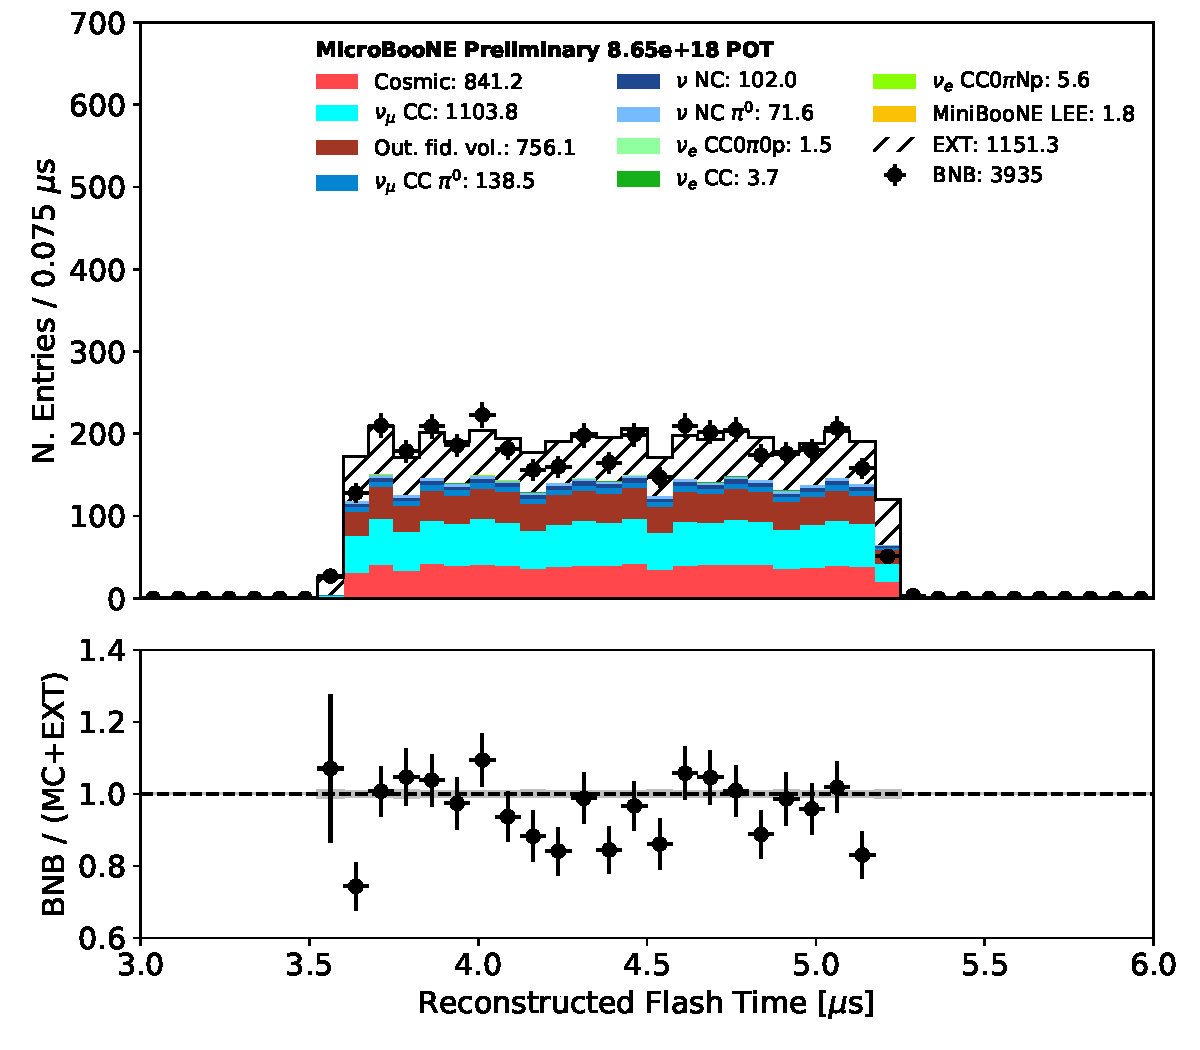
\includegraphics[width=1.00\textwidth]{NuId-Ch3/Images/flash_time_01152020_CRT.pdf}
    \caption{\label{fig:crt:post} With CRT tools.}
    \end{subfigure}
\caption{\label{fig:crt} Beam timing distribution before (a) and after (b) CRT tools have been applied. The EXT contribution is reduced by over a factor of three.}
\end{center}
\end{figure}
